\documentclass{article}
\usepackage[margin=1in]{geometry}
\usepackage{graphicx}
\usepackage{amsmath}
\usepackage{multirow}
\usepackage{multicol}
\usepackage{wrapfig}



%\topmargin 0pt
%\oddsidemargin 12pt
%\evensidemargin 12pt
\interfootnotelinepenalty=10000


\begin{document}
\title{Partial Confidence in DNA Sequence Alignment}
\author{Yi Tian Xu\\260520039}

\maketitle

\abstract{}

%\begin{multicols}{2}

\section{Introduction}

\section{Method}

\subsection{Similarity measure}

Classical sequence alignment is based on a dynamic programming that computes some similarity measure for each pair of nucleotides of the input sequences. The similarity measure generally scores according to the likeness of the substitution, insertion and deletion. In our method, we use $m = 2$ for identity, $s_t = -1$ for transition and $s_v = -2$ for transversion substitutions, and a linear gap function $g(x)=-2x$. To formalize the substitution score, let $M$ be the substitution matrix. 
\begin{equation}
	M = \begin{bmatrix}
		m & s_v & s_t & s_v\\
		s_v & m & s_v & s_t\\
		s_t & s_v & m & s_v\\
		s_v & s_t & s_v & m\\
	\end{bmatrix}
\end{equation}
Given the alphabet $\Sigma =$ \{A,C,G,C\}, we can represent a nucleotide $a \in \Sigma$ as a vector $\vec{u}_a = (u_{\mbox{A}}, u_{\mbox{C}}, u_{\mbox{G}}, u_{\mbox{T}})$ where each entry $u_x = 1$ if $x = a$ or 0 otherwise. Thus, the score for matching two nucleotides, $a$ and $b$ can be formulate as $s(a,b) = \vec{u}_aM\vec{u}_b$.

To induce the probabilistic property in the reference sequence, we modify the similarity measure as the following. Given the reference nucleotide $a$ and its confidence probability $p$, we construct the vector $\vec{u}_{a,p} = (u_{\mbox{A}}, u_{\mbox{C}}, u_{\mbox{G}}, u_{\mbox{T}})$ where each entry $u_x = p$ if $x=a$ or $(1-p)/3$ otherwise. The score for matching a query nucleotide $b$ is $s(a,b,p) = \vec{u}_{a,p}M\vec{u}_b$. We can see that this preserves the scores in the total confidence setting since when $p=1$, $u_{a,p} = u_a$ for all $a \in \Sigma$. 

For the chosen parameters $m, s_t$ and $s_v$, Figure \ref{figure:score_graphs} shows the substitution score according to the variation in the confidence $p$. 

\begin{wrapfigure}{r}{0.5\textwidth}
\begin{center}
\caption{Substitution score variation according to the confidence value.}
   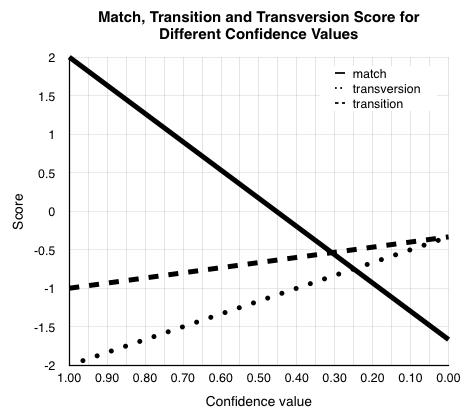
\includegraphics[width=0.5\textwidth]{score_graph}
\label{figure:score_graphs}
\end{center}
\end{wrapfigure}

\subsection{Indexing}

To search in a long gene sequence $G$ of thousands of nucleotides, basic local alignment search tool (BLAST) indexes the reference sequence by a list of high-scoring $w$-mers. The steps in searching the alignment of a query sequence $q$ therefore consists of splitting $q$ into $w$-mers, searching for their occurrence in the $G$ and extend the alignment. 

\subsection{Implementation}

\section{Experiment}
\subsection{Global Alignment}

\subsection{Local Alignment}
%\end{multicols}

\end{document}